\subsubsection*{Informazioni sul package}
\begin{figure}[h]
	\centering
	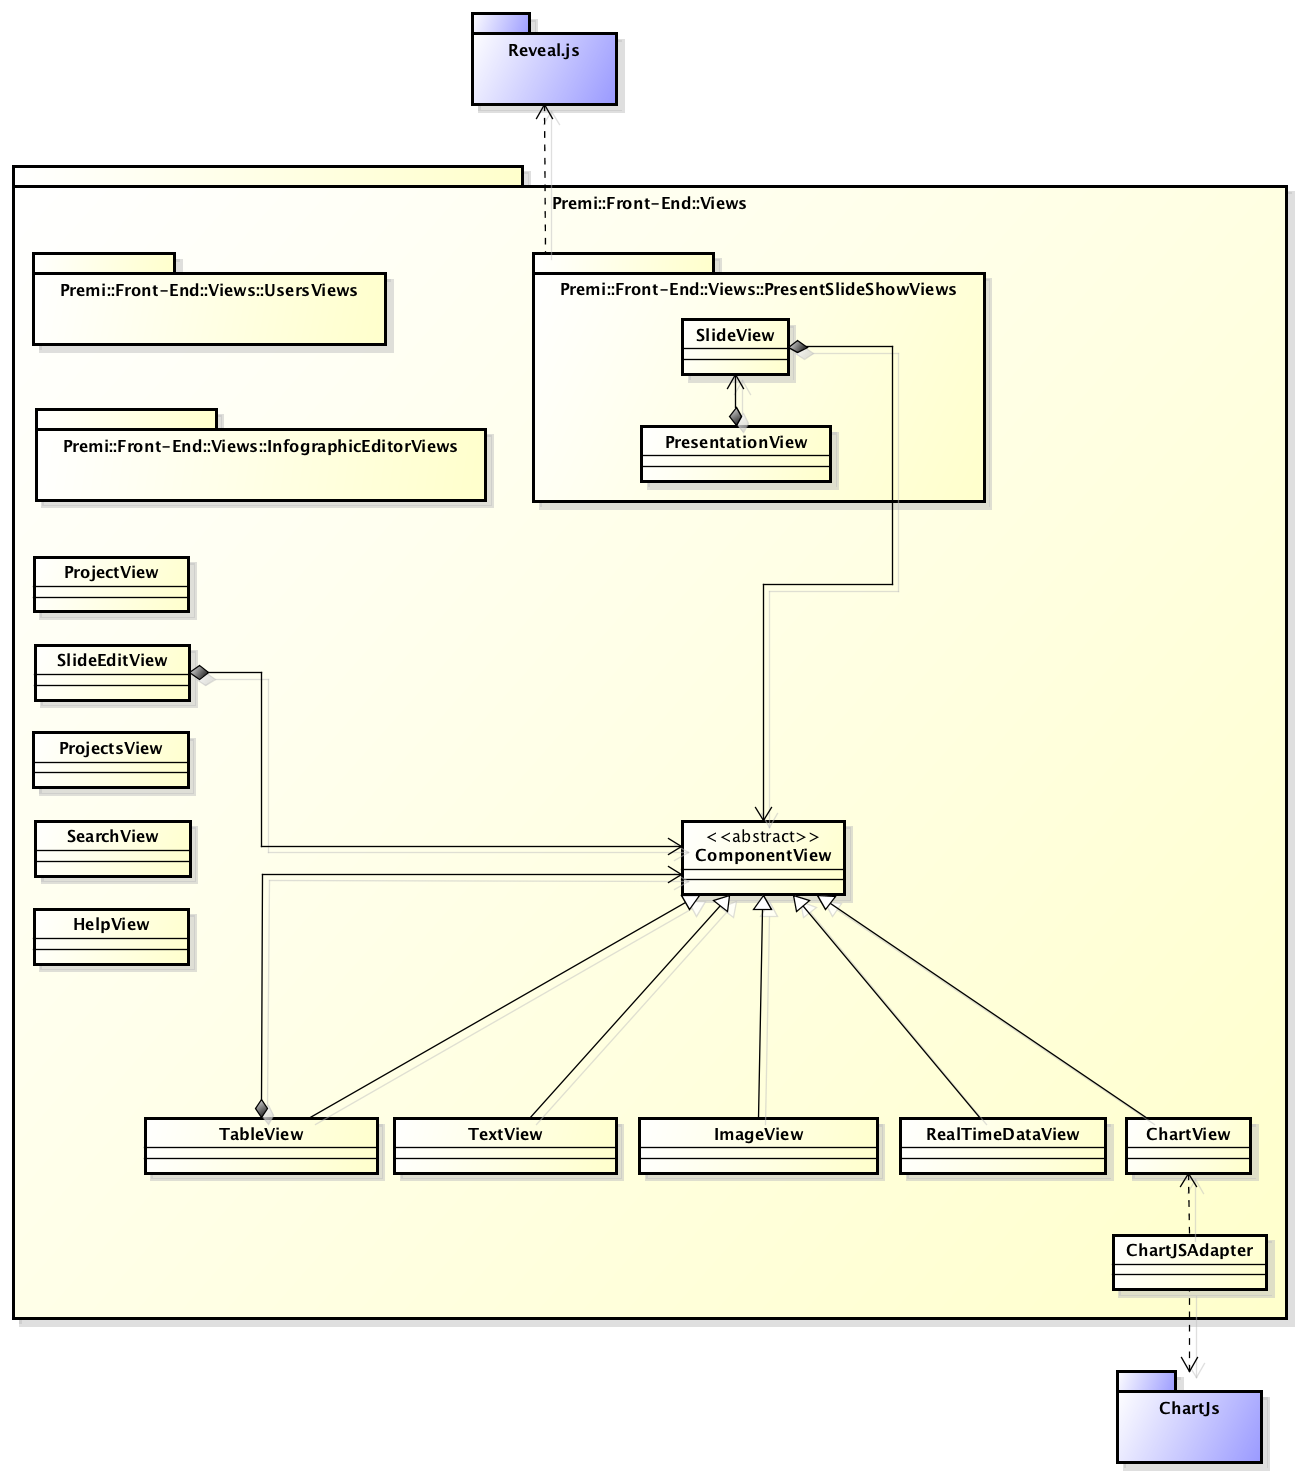
\includegraphics[width=0.9\linewidth]{img/front-end_views}
	\caption[Premi::Front-End::Views]{Premi::Front-End::Views}
\end{figure}
Il package contiene gli elementi per creare la parte grafica del \gls{front-end}, la visualizzazione delle pagine e dell'editor del progetto.

\subsubsection*{Classi contenute:}
\begin{itemize}

	\item Premi::Front-End::Views::HomePageView:
	\begin{itemize}
		\item \textbf{Descrizione}: classe per la gestione della pagina iniziale del sito.
	\end{itemize}

	\item Premi::Front-End::Views::LoginView:
	\begin{itemize}
		\item \textbf{Descrizione}: classe per la gestione della pagina per l'accesso al sito e il recupero delle proprie credenziali.
	\end{itemize}

	\item Premi::Front-End::Views::SignUpView:
	\begin{itemize}
		\item \textbf{Descrizione}: classe per la gestione della pagina per la registrazione al sito.
	\end{itemize}

	\item Premi::Front-End::Views::ProjectsView:
	\begin{itemize}
		\item \textbf{Descrizione}: classe per la gestione della pagina contenente i progetti creati da un utente.
	\end{itemize}

	\item Premi::Front-End::Views::HelpView:
	\begin{itemize}
		\item \textbf{Descrizione}: classe per la gestione della guida all'applicazione.
	\end{itemize}

	\item Premi::Front-End::Views::PresentationView:
	\begin{itemize}
		\item \textbf{Descrizione}: classe per la gestione della visualizzazione della presentazione.
	\end{itemize}

	\item Premi::Front-End::Views::PresentationEditorView:
	\begin{itemize}
		\item \textbf{Descrizione}: classe per la gestione della pagina dell'editor della presentazione.
	\end{itemize}

	\item Premi::Front-End::Views::SlideEditorView:
	\begin{itemize}
		\item \textbf{Descrizione}: classe per la gestione della pagina dell'editor di una \gls{slide};
		\item \textbf{Relazioni con altre classi}:
		\begin{itemize}
			\item Premi::Front-End::Views::ComponentView.
		\end{itemize}
	\end{itemize}

	\item Premi::Front-End::Views::ComponentsView:
	\begin{itemize}
		\item \textbf{Descrizione}: classe per la gestione grafica degli elementi che è possibile includere in una \gls{slide}.
	\end{itemize}

	\item Premi::Front-End::Views::InfographicView:
	\begin{itemize}
		\item \textbf{Descrizione}: classe per la gestione dell pagina per l'\gls{infografica}.
	\end{itemize}

\end{itemize}
